Um dynamisch später hinzugefügte Algorithmen auch in der Ein- und Ausgabe zu unterstützen, werden die Komponenten "`PluginLoader"' und "`Plugin"' verwendet. Der PluginLoader handhabt die Plugins und erstellt diese falls notwendig. Um dies zu tun, hat der PluginLoader Zugriff auf die Algorithmen. Somit kann der PluginLoader ein Plugin für die Eingabe von Parametern erzeugen, indem er sich von dem entsprechenden Algorithmus die Anzahl der benötigten Parameter ausgeben lässt. Analog kann der PluginLoader ein Plugin zur Ausgabe erzeugen, indem er sich zurückgeben lässt wie die Ausgabedaten aussehen und diese Anhand des gewünschten Ausgabeformats entweder als plain-text, html-text, JSON, PNG-Grafik oder SVG+XML-Grafik aufbereitet.\\
\begin{figure}[h]
\centering
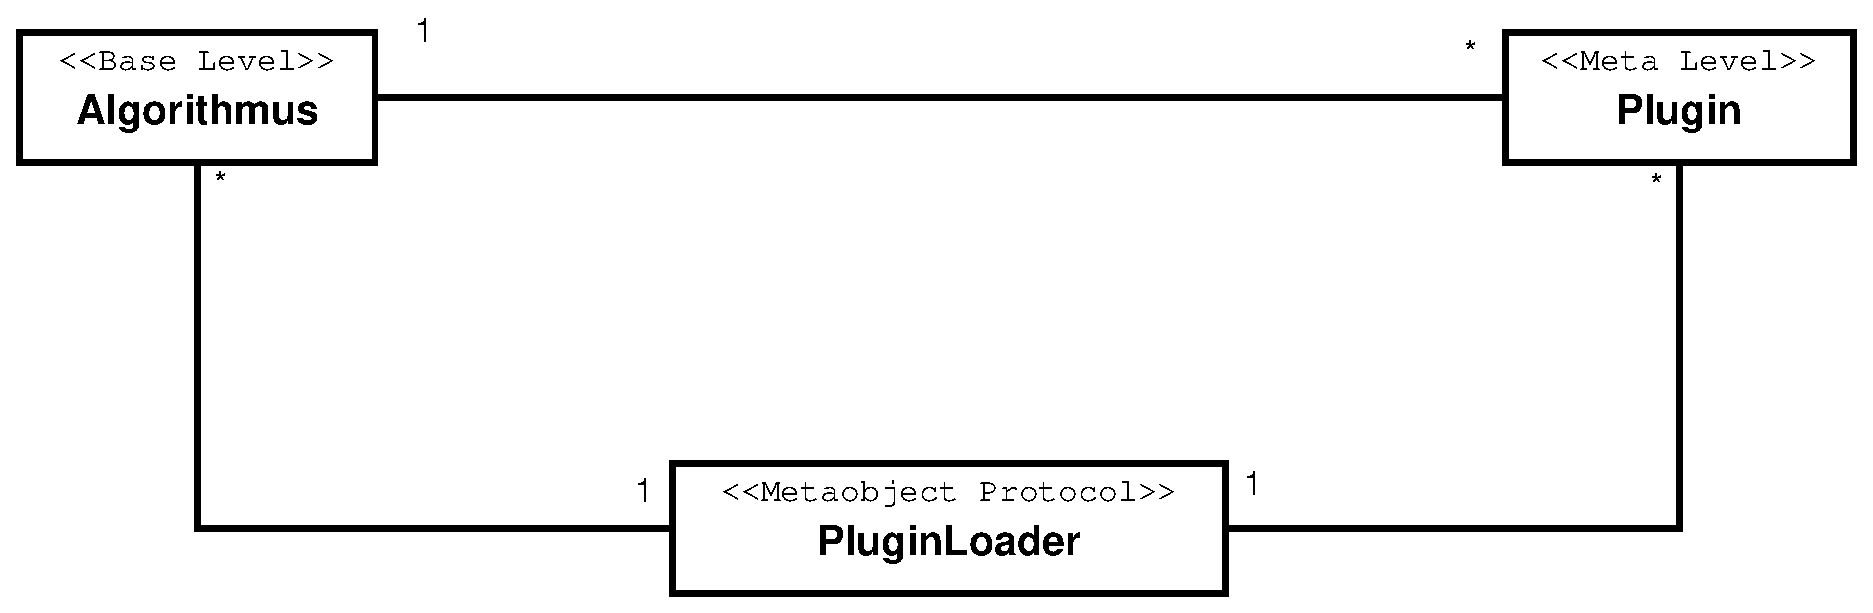
\includegraphics[width=0.9\linewidth]{Grafik/Diagramm/Reflection}
\caption[Reflection-Klasse]{Reflectoin-Pattern mit PluginLoader}
\label{fig:Reflection}
\end{figure}

